\documentclass[runningheads]{llncs}

%% Some recommended packages.
\usepackage{booktabs}   %% For formal tables:
                        %% http://ctan.org/pkg/booktabs
% \usepackage{subcaption} %% For complex figures with subfigures/subcaptions
                        %% http://ctan.org/pkg/subcaption
\usepackage{multirow}

\usepackage{listings}

\usepackage{graphicx}

\usepackage{proof}

\usepackage{amsmath}

\usepackage{xcolor}

\usepackage{xspace}
\newcommand{mk}{\textsc{miniKanren}}

\sloppy
% Used for displaying a sample figure. If possible, figure files should
% be included in EPS format.
%
% If you use the hyperref package, please uncomment the following line
% to display URLs in blue roman font according to Springer's eBook style:
% \renewcommand\UrlFont{\color{blue}\rmfamily}

\graphicspath{{figures/}}

\setlength{\textfloatsep}{5pt}
\setlength{\belowcaptionskip}{-3pt}
\setlength{\abovecaptionskip}{0pt}

\setlength{\abovedisplayskip}{-3pt}
\setlength{\belowdisplayskip}{-2pt}
\setlength{\abovedisplayshortskip}{0pt}
\setlength{\belowdisplayshortskip}{2pt}

\begin{document}

\title{An Empirical Study of Partial Deduction for \mk}

%
%\titlerunning{Abbreviated paper title}
% If the paper title is too long for the running head, you can set
% an abbreviated paper title here
%
\author{Anonymous author(s)}
%
\authorrunning{Anonymous author(s)}
% First names are abbreviated in the running head.
% If there are more than two authors, 'et al.' is used.
%
\institute{Anonymous institute(s)}


\maketitle

\begin{abstract}
  We explore partial deduction for \mk: a specialization technique aimed at improving the performance of a relation in the given direction.
  We describe a novel approach to specialization of \mk based on partial deduction and supercompilation.
  On several examples, we demonstrate issues which arise during partial deduction.
\end{abstract}


\section{Introduction}

The core feature of the family of relational programming languages \mk\footnote{\mk language web site: \url{http://minikanren.org}} is their ability to run a program in different directions.
Having specified a relation for adding two numbers, one can also compute the subtraction of two numbers or find all pairs of numbers which can be summed up to get the given one.
Program synthesis can be done by running \emph{backwards} a relational interpreter for some language.
In general, it is possible to create a solver for a recognizer by translating it into \mk and running in the appropriate direction~\cite{lozov2019relational}.

The search employed in \mk is complete which means that every answer will be found, although it may take a long time.
The promise of \mk falls short when speaking of performance.
The running time of a program in \mk is highly unpredictable and varies greatly for different directions.
What is even worse, it depends on the order of the relation calls within a program.
One order can be good for one direction, but slow down the computation drastically in the other direction.

Specialization or partial evaluation~\cite{jonesbook} is a technique aimed at improving the performance of a program given some information about it beforehand.
It may either be a known value of some argument, its structure (i.e. the length of an input list) or, in case of a relational program, --- the direction in which it is intended to be run.
An earlier paper~\cite{lozov2019relational} showed that \emph{conjunctive partial deduction}~\cite{de1999conjunctive} can sometimes improve the performance of \mk programs.
Unfortunately, it may also not affect the running time of a program or even make it slower.

Control issues in partial deduction of logic programming language \pro have been studied before~\cite{leuschel2002logic}.
The ideas described there are aimed at left-to-right evaluation strategy of \pro.
Since the search in \mk is complete, it is safe to reorder some relation calls within the goal for better performance.
While sometimes conjunctive partial deduction gives great performance boost, sometimes it does not behave as well as it could have.

In this paper, we show on examples some issues which conjunctive partial deduction faces.
We also describe a novel approach to partial deduction of a relational programming language \mk.
We compare it to the existing specialization algorithm on several programs and discuss why some \mk programs run slower after specialization.

\section{Related Work}

Specialization is an attractive technique aimed to improve the performance of a program if some of its arguments are known statically.
Specialization is studied for functional, imperative and logic programing and comes in different forms: partial evaluation~\cite{jonesbook} and partial deduction~\cite{lloyd1991partial}, supercompilation~\cite{soerensen1996positive}, distillation~\cite{hamilton2007distillation} and many more.


The heart of supercompilation-based techniques is \emph{driving}~---~a symbolic execution of a program through all possible execution paths.
The result of driving is so-called \emph{process tree} where nodes correspond to \emph{configurations} which represent computation state.
For example, in the case of pure functional programming languages, the computational state might be a term.
Each path in the tree corresponds to some concrete program execution.
The two main sources for supercompilation optimizations are aggressive information propagation about variables' values, equalities and disequalities, and precomputing of all deterministic semantic evaluation steps.
The latter process, also known as \emph{deforestation}~\cite{deforestation}, means  combining of consecutive process tree nodes with no branching.
When the tree is constructed, the resulting, or \emph{residual}, program can be extracted from the process tree by the process called \emph{residualization}.
Of course, process tree can contain infinite branches.
\emph{Whistles} --- heuristics to identify possibly infinite branches --- are used to ensure supercompilation terminates.
If a whistle signalls during the construction of some branch, then something should be done to ensure termination.
The most common approaches include stop driving the infinite branch completely (no specialization is done in this case and the source code is blindly copied into the residual program) or fold the process tree to a \emph{process graph}.
The main instrument to perform such a folding is \emph{generalization}.
Generalization, abstracting away some computed data about the current term, makes folding possible.
%  i.e. abstracting away some computed data about the current term which makes folding possible.
One source of infinite branches is consecutive recursive calls to the same function with an accumulating parameter: by unfolding such a call further one can only increase the term size which leads to nontermination.
The accumulating parameter can be removed by replacing the call with its generalization.
There are several ways to ensure process correctness and termination, most-specific generalization
(anti-unification) and using \emph{homeomorphic embedding}~\cite{Higman52,Kruskal60} as a
whistle being the most common.
%the most common being \emph{homeomorphic embedding}~\cite{Higman52,Kruskal60} used as a whistle and most-specific generalization of terms.
% When two dangerously similar nodes are encountered,
% For example, two consecutive recursive calls of a function with accumulating parameter, and the first is not an instance of the second, then one may construct a new, generalized, node such that both of original nodes are instances of the last one, then one of the initial nodes is replaced with the generalized one.

While supercompilation generally improves the behaviour of input programs and distillation can even provide superlinear speedup, there are no ways to predict the effect of specialization on a given program in the general.
What is worse, the efficiency of residual program from the target language evaluator point of view is rarely considered in the literature.
The main optimization source is computing in advance all possible intermediate and statically-known semantics steps at program transformation-time.
Other criteria, like the size of the generated program or possible optimizations and execution cost of different language constructions by the target language evaluator, are usually out of consideration~\cite{jonesbook}.
It is known that supercompilation may adversely affect GHC optimizations yielding standalone compilation more powerful~\cite{SCBE,TCES} and cause code explosion~\cite{SCHC}.
Moreover, it may be hard to predict the real speedup of any given program on concrete examples even disregarding the problems above because of the complexity of the transformation algorithm.
The worst-case for partial evaluation is when all static variables are used in a dynamic context, and there is some advice on how to implement a partial evaluator as well as a target program so that specialization indeed improves its performance~\cite{jonesbook,bulyonkov84}.
There is a lack of research in determining the classes of programs which transformers would definitely speed up.

Conjunctive partial deduction~\cite{de1999conjunctive} makes an effort to provide reasonable control for the left-to-right evaluation strategy of \pro.
CPD constructs a tree which models goal evaluation and is similar to a SLDNF tree, then a residual program is generated from this tree.
Partial deduction itself resembles driving in supercompilation~\cite{gluck1994partial}.
The specialization is done in two levels of control: the local control determines the shape of the residual programs, while the global control ensures that every relation which can be called in the residual program is indeed defined.
The leaves of local control trees become nodes of the global control tree.
CPD analyses these nodes at the global level and runs local control for all those which are new.

At the local level, CPD examines a conjunction of atoms by considering each atom one-by-one from left to right.
An atom is \emph{unfolded} if it is deemed safe, i.e. a whistle based on homeomorphic embedding does not signal for the atom.
When an atom is unfolded, a clause whose head can be unified with the atom is found, and a new node is added into the tree where the atom in the conjunction is replaced with the body of that clause.
If there is more than one suitable head, then several branches are added into the tree which corresponds to the disjunction in the residualized program.
An adaptation of CPD for the \mk programming language is described in~\cite{lozov2019relational}.

\ecce partial deduction system~\cite{leuschel1997ecce} is the most mature implementation of CPD for \pro.
\ecce provides various implementations of both local and global control as well as several degrees of post-processing.
Unfortunately there is neither an automatic procedure to choose what control setting is likely to improve input programs the most nor any informal recommendations on how to choose the best settings.
The choice of the proper control is left to the user.

An empitical study shown that the most well-behaved strategy of local control in CPD for \pro is \emph{deterministic unfolding}~\cite{leuschel1997advanced}.
An atom is unfolded only if precisely one suitable clause head exists for it with the one exception: it is allowed to unfold an atom non-deterministically once for one local control tree.
This means that if a non-deterministic atom is the leftmost within a conjunction, it is most likely to be unfolded and to introduce many new relation calls within the conjunction.
We believe this is the core problem with CPD which limits its power when applied to \mk.
The strategy of unfolding atoms from left to right is reasonable in the context of \pro because it mimics the way programs in \pro execute.
But it often leads to larger global control trees and, as a result, bigger, less efficient programs.
The evaluation result of a \mk program does not depend on the order of atoms (relation calls) within a conjunction, thus we believe a better result can be achieved by selecting a relation call which can restrict the number of branches in the tree.
We describe our approach which implements this idea in the next section.

\newcommand{\code}[1]{\texttt{#1}}

\section{Non-conjunctive Partial Deduction}

In this section we describe a novel approach to specialization of relational programs.
This approach draws inspiration from both conjunctive partial deduction and supercompilation.
The aim was to create a specialization algorithm which is simpler than conjunctive partial deduction and uses properties of \mk{} to improve performance of the input programs.

The algorithm pseudocode is shown on Fig.~\ref{fig:ncpd-pseudo}.
For the sake of brevity and clarity, we provide functions \code{drive\_disj} and \code{drive\_conj} which describe how to process disjunctions and conjunctions respectively.
Driving itself is a trivial combination of presented functions (line 2).

A driving process creates a process tree, from which a residual program is later created.
The process tree is meant to mimic the execution of the input program.
The nodes of process tree include a \emph{configuraion} which describes the state of program evaluation at some point.
In our case configuration is a conjunction of relation calls.
The substitution computed at each step is also stored in the tree node, although it is not included into the configuration.

Hereafter, we consider all goals and relation bodies to be in \emph{canonical normal form}~---~a disjunction of conjunctions of either calls or unifications.
Moreover, we assume all fresh variables to be introduced into scope and all unifications to be computed at each step.
Those disjuncts in which unifications fail are removed.
Other disjuncts take form of a conjunction of relation calls accompanied with a substitution computed from unificaitons.
Any miniKanren term can be trivially transformed to the described form.
In Fig.~\ref{fig:ncpd-pseudo} function \code{normalize} is assumed to perform term normalization.
The code is omitted for brevity.

\begin{figure}[!t]
  \centering
  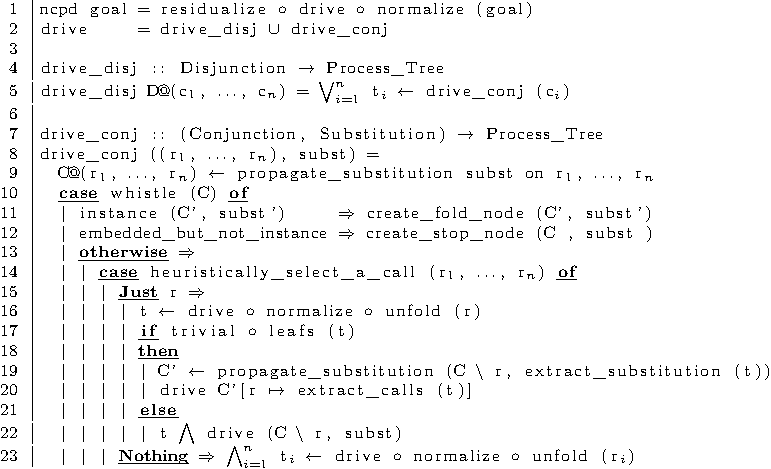
\includegraphics[width=0.85\textwidth]{algo_pseudo-crop.pdf}
  \caption{\db{Non-conjunctive Partial Deduction Pseudo Code}}
  \label{fig:ncpd-pseudo}
\end{figure}

% The very first step of driving a conjunction is to apply a substitution to the variables in relation calls (line 10).

There are several core ideas behind this algorithm.
The first is to select an arbitrary relation to unfold, not necessarily the leftmost which is safe.
The second idea is to use a heuristic which decides if unfolding a relation call can lead to discovery of contradictions between conjuncts which in turn leads to restriction of the answer set at specialization-time \db{(line 14; \code{heuristically\_select\_a\_call} stands for heurictics combination, see section~\ref{sec:heurictic} for details)}.
If those contradictions are found, then they are exposed by considering the conjunction as a whole and substituting the result of the call unfolding back into the conjunction the call was selected from thus \emph{joining} the conjunction back together instead of using \emph{split} as in CPD \db{(lines 15--22)}.
Finally, if the heuristic fails to select a potentially good call, then the conjunction is splitted into individual calls which are driven in isolation and are never joined \db{(line 23)}.

When the heuristic selects a call to unfold (line \db{15}), a process tree is constructed for the selected call \emph{in isolation} (line \db{16}).
The leaves of the computed tree are examined.
If all leaves are either computed substitutions or are renamings of some relations accompanied with non-empty substitutions, then the leaves are collected and replace the considered call in the root conjunction (lines \db{19--20}).
If the selected call does not suit the criteria, the results of its unfolding is not propagated onto other relation calls withing the conjunction and the next suitable call is selected (line \db{22}).
According to the denotational semantics of \mk{} it is safe to compute individual conjuncts in any order, thus it is ok to drive any call and then propagate its results onto the other calls.

% Each time we examine a conjunction of calls, we \emph{split} them into separate nodes which are driven independently from each other.
% Among the relation calls we select one which is according to the heuristic is likely to narrow down the answer set \db{(line 15)}.
% If the selected call does not suit the criteria, the results of its unfolding is not propagated onto other relation calls withing the conjunction and the next suitable call is selected \db{(line 22)}.

This process creates branchings whenever a disjunction is examined lines 4--\db{5}).
At each step we make sure that we do not start driving a conjunction which we have already examined.
To do this, we check if the current conjunction is renaming of any other configuration in the tree (line \db{11}).
If it is, then we create a special node which then is residualized into a call to the corresponding relation.
This is known as \emph{folding} in supercompilation.

We decided not to perform generalization in this approach in the same fashion as CPD or supercompilation does.
Our conjunctions are always splitted into individual calls and are joined back together if it is sensible.
If the need for generalization arises, i.e. embedding is detected, then we immediately stop driving this conjunction (line \db{12}).
When redisualizatin such conjunction, we just generate a conjunction of calls to the input program before specialization.

% The generalization is used in supercompilation and partial deduction to ensure termination at the same time as some degree of specialization.
% The generalization of two terms is usually a \emph{most-specific generalization}.
% Generalization is used to abstract away some information computed during driving.
% In conjunctive partial deduction generalization is modified to support treating of conjunctions.
% The generalization selects subconjuctions of two conjuncts which are similar (call to the same relation and their arguments have similar shape and distribution).
% For the subconjunctions selected a most-specific generalization is computed.

% In our approach we only do splitting of a conjunction into individual relation calls.
% This makes any program with an accumulating parameter to be a problem.
% Sometimes when there is a need to do a proper generalization, it is in reality just an instance of some other goal within the tree and we can simply create a call there \db{(line 13)}.
% Otherwise we are unable to meaningfully specialize such goal, but we can always just include the initial program in the residual program and call the corresponding relation.


\subsection{Unfolding}

Unfolding in our case is done by substitution of some relation call by its body with simultaneous normalization and computation of unifications.
% To unfold a relation call we do the following steps.
% \db{TODO: the following has alredy mentioned above.}
% First, the formal arguments of a relation are substituted for the actual arguments of the call in the body.
% All fresh variables get instantiated.
% The body is transformed into a canonical form (disjunction of conjunctions of either calls or unifications).
% All unifications are computed.
% Those disjuncts in which unifications fails are removed.
% Other disjuncts take form of a conjunction of relation calls accompanied with a substitution.
The unfolding itself is straightforward however it is not always clear what to unfold and when to \emph{stop} unfolding.
Unfolding in functional programming languages specialization, as well as inlining in imperative one, is usually considered to be safe from a residual program efficiency point of view.
It may only lead to code explosion or code duplication which is mostly left to a target program compiler optimization or even is out of consideration at all if a specializer is considered as a standalone tool~\cite{jonesbook}.

Unfortunately, this is not the case for the specialization of relational programming language.
Unlike functional and imperative, in logic and relational programming language unfolding may easily affect the target program efficiency~\cite{leuschel2002logic}.
Unfolding too much may create extra unifications, which is by itself a costly operation, or even introduce duplicated computations by propagating the unfolding results onto neighboring conjuncts.

There is a fine edge between too much unfolding and not enough unfolding.
The former may be even worse than the latter.
We believe that the following heuristic provides a reasonable approach to controling unfolding.

\subsection{Heuristic}
\label{sec:heurictic}

This heuristic is aimed at selecting the relation call within a conjunction which is both safe to unfold and may lead to discovering contradictions within the conjunction.
The unsafe unfolding leads to uncontrollable increase in the number of relation calls in a conjunction.
It is best to first unfold those relation calls which can be fully computed up to substitutions.

We deem every static conjunct (non-recursive) to be safe because they never lead to growth in the number of conjunctions.
Those calls which unfold deterministically, meaning there is only one disjunct in the unfolded relation, are also considered to be safe.

The other part of heuristic is less trivial, we call it the branching heuristic.
It considers the case when the unfolded relation contains less disjuncts than it could possibly have.
This means that we found some contradiction, some computations were gotten rid of, and thus the answer set was restricted, which is desirable when unfolding.
To compute this heuristic we precompute the maximum possible number of disjuncts in each relation and compare this number with the number of disjuncts when unfolding a concrete relation call.
Maximum number of disjuncts is computed by unfolding the body of the relation in which all relation calls were replaced by a unification which always succeeds.

\begin{figure}[h!]
  \centering
  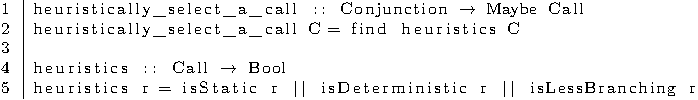
\includegraphics[width=0.75\textwidth]{heuristic-crop.pdf}
  \caption{Heuristic selection pseudocode}
  \label{fig:heu-pseudo}
\end{figure}

%  more complicated case is when there are less disjuncts than there can possibly be.
% This signifies that at least one branch of computations is gotten rid of.

The pseudocode describing heuristic is shown in fig.~\ref{fig:heu-pseudo}.
Selecting a good relation call can fail (line 1).
The implementation works such that we first select those relation calls which are static, and only if there are none, we proceed to look at deterministic unfoldings and then we search for those which are less branching.
This heuristic provides a good balance in unfolding.
% The final heuristic selects the first conjunct which suites either of the following cases.
% First we unfold those conjuncts which are static.
% Then --- deterministic.
% Then those which are less branching.
% The last to be unfolded are those calls, which unfold to a substitution with not conjunction.

% \subsection{Residualization}

% Residualization is quite straightforward.
% A branching in the process tree becomes a disjunction.
% A split node becomes a conjunction.
% Computed substitution is residualized as a conjunction of unifications.
% A renaming node is just a call to a relation.
% Relations are created for configurations on which leaf nodes are renamed.

% One other thing is that when some configuration is occurred within the tree which is an instance of a configuration for which a new relation is created, then we just create a call.

\section{Evaluation}
In our study we compared the new conservative partial deduction with the \ecce partial deduction system.
\ecce is designed for \pro programming language and cannot be directly applied to \mk.
To be able to compare our approach with \ecce, we converted each input program first to the pure subset of \pro, then transformed it with \ecce, and then we converted the result back to \mk.
The coversion to \pro is a simple syntactic conversion.
In conversion from \pro to \mk, a conjunction is generated by each horn clause in which unifications are placed before any relation call.
This mimics in \mk the execution order of \pro program within a conjunction.

The set of benchmarks consist of both examples from the literature on partial deduction and programs of our own creation.
The first two programs are well-known in conjunctive partial deduction literature~\cite{de1999conjunctive}.
The second two are introduced in the paper on relational interpreters~\cite{lozov2019relational}.
The last two are examples of relational interpreters created by us which are observable, but non-trivial.
In the last two examples we explore how different implementations of the same relation affects the quality of transformations.

The \lstinline{doubleAppend$^o$} program concatenates three lists of numbers by computing a conjunction of two calls of a relation which concatenates two lists.
This example is prominent in CPD literature, since it demonstrates \emph{deforestation} --- a transformation which gets rid of intermidiate datastructures.
This transformation cannot be done with the earlier partial deduction approach, since the relation uses a variable shared between two relation calls within a conjunction which requires the transformation to treat conjunctions as a whole.
We explore how the fact that our approach sometimes splits conjunctions ignoring the variable sharing affects the quality of transformation.

The \lstinline{maxLength$^o$} program computes the maximum element of the list as well as its length.
In this program an input list is shared between the call of the relation to compute the maximum element and the relation to compute the length of the list.
This sharing leads to the list being traversed twice during execution.
This example is used to demonstrate \emph{tupling}: the transformation in which multiple traversals of the same data structure are replaced with a single traversal which computes all the necessary results simultaneously.
CPD performes tupling more often than our approach, and we explore how it affects the performance of the transformed program.

The \lstinline{isPath} and \lstinline{unify} relations demonstrate the relation interpretation approach in which a relation is generated from a functional program.
Partial deduction is capable to improve the execution time of the generated relations in the given direction.
These two relations are described in~\cite{lozov2019relational} thus we will only briefly describe them in this paper.
Here the aim is to study if our approach can help to achieve comparable performance improvement as \ecce.

The \lstinline{eval$^o$} relation implements an evaluator of a subset of propositional formulas.
We consider four different implementations of this relation to explore how the way program is implemented can affect the quality of transformation.
Depending on the implementation, \ecce generates programs of varying performance, while the execution time of the program generated by our approach is similar.

The \lstinline{typecheck$^o$} relation implements a typechecker for a tiny expression language.
We consider two different implementations of this relation: one written by hand and the other generated from the functional program.
We demonstrate how much these implementations differ in terms of performance before and after transformations.

In this study we only measured the execution time for the sample queries, averaging them over multiple runs.
All examples of \mk relations in this paper are written in \oc\footnote{\oc: statically typed \mk embedding in \ocaml. The repository of the project: \url{https://github.com/JetBrains-Research/OCanren}}.
The queries were run on a laptop running Ubuntu 18.04 with quad core Intel Core i5 2.30GHz CPU and 8 GB of RAM.

The tables and graphs use the following denotations.
\emph{Original} represents the execution time of a program before any transformations were applied; \emph{ECCE} --- of the program transformed with \ecce with default conjunctive control setting; \emph{ConsPD} --- of the program transformed by our approach.
The first two examples also contain \emph{Ideal} row which contain the execution time of the ideal implementations of the relations presented in the paper~\cite{de1999conjunctive}.

\subsection{Concatenation of Three Lists}

The relation \lstinline{doubleAppend$^o$} concatenates three lists by a conjunction of two calls of the \lstinline{append$^o$} relation (see fig.~\ref{doubleApp}).
These two calls share a variable --- an intermediate list \lstinline{ts}.
The list \lstinline{xs} is traversed twice to construct the result: first when \lstinline{ts} is constructed and then, when \lstinline{ts} is traversed during the second call.
This double traversal negatively impacts the execution time, but it can be removed by deforestation.

\begin{figure*}[!h]
  \centering
  \begin{minipage}{0.6\textwidth}
    \begin{lstlisting}[label={doubleApp}, caption={Concatenation of three lists}, captionpos=b, frame=tb]
  let doubleAppend$^o$ xs ys zs res =
    fresh (ts) (
      append$^o$ xs ys ts /\ append$^o$ ts zs res)

  let rec append$^o$ xs ys zs = conde [
    (xs === [] /\ ys === zs);
    fresh (h t r) (
      xs === (h % t) /\
      zs === (h % r) /\
      append$^o$ t ys r)]
    \end{lstlisting}
  \end{minipage}
\end{figure*}

The better implementation of this relation (see fig.~\ref{doubleApp:ideal}) does not traverse the first list twice.
It first recursively copies \lstinline{xs} into the beginning of \lstinline{res}, and only when \lstinline{xs} is fully consumed, it calls the \lstinline{append$^o$} to concatenate \lstinline{ys} and \lstinline{zs}.
This implementation is provided as the ideal implementation of \lstinline{doubleAppend$^o$} in~\cite{de1999conjunctive}.

\begin{figure*}[!h]
  \centering
  \begin{minipage}{0.6\textwidth}
    \begin{lstlisting}[label={doubleApp:ideal}, caption={Ideal implementation of concatenation of three lists}, captionpos=b, frame=tb]
  let doubleAppend$^o$ xs ys zs res = conde [
    (xs === [] /\ append$^o$ ys zs res);
    fresh (h t r) (
      xs === h % t /\
      res === h % r /\
      doubleAppend$^o$ t ys zs r)]
    \end{lstlisting}
  \end{minipage}
\end{figure*}

To automatically transform the initial program into the ideal implementation, the transformer should treat the conjuncts which share variables with care.
Partial deduction splits any conjunction into its subconjunctions, regardless variable sharing, while CPD only splits conjunctions when potential non-termination is detected.
Conservative partial deduction processes subconjunctions in isolation and then joins them back together, if it can help to restrict the search space.
In this example, ConsPD fails to perform deforestation: ConsPD first splits the conjunction \lstinline{append$^o$ xs ys ts /\ append$^o$ ts zs rs} into two relation calls of \lstinline{append$^o$}, then unfolds the first call, but since the second call is a renaming of the first one, it is not unfolded.
The generated program is almost the same as the original: the only difference being that the fresh variables are introduced on the toplevel.


We run all programs in the forward and the backward direction.
The forward direction \lstinline{doubleAppend$^o$ x y z ?} concatenates three given lists: the first one of length 700, the second and the third --- of length 1.
The backward direction \lstinline{doubleAppend$^o$ ? ? ? r} searches for the first 100 list triples whose concatenation gives the given list of length 700.

\begin{table}
  \centering
  \begin{tabular}{c||c||c}
                  & forward & backward \\
  \hline\hline
  Original        & 34.8ms & 1.6ms \\ \hline
  \ecce           & 26.7ms & 1.7ms \\ \hline
  Ideal           & 26.9ms & 1.7ms \\ \hline
  ConsPD         & 47.6ms & 1.7ms
  \end{tabular}
  \caption{Evaluation results for doubleAppendo}
  \label{tbl:doubleApp}
\end{table}

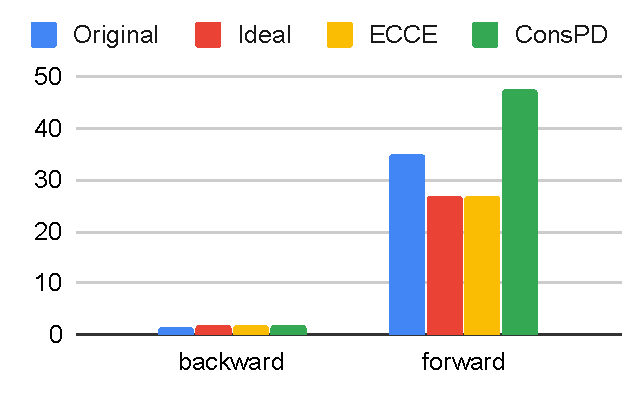
\includegraphics{graphs/doubleApp.pdf}

There is no significant difference in the execution time in the backward direction between different specialized versions (see table~\ref{tbl:doubleApp}).
However the execution time in the backward direction differs: the program generated by \ecce shows the same speedup as the ideal program, while conservative partial deduction slows the program down.
The reason behind the slowdown is the premature introduction of fresh variables which is significant for the input data of this size.

\subsection{Maximum Element and Length of a List}

The relation \lstinline{maxLenght$^o$} computes the maximum element of the input list and its length (see fig.~\ref{cpd:maxandlength}) by conjunction of two relation calls.
The list \lstinline{xs} is traversed twice: first to compute the maximum in the relation \lstinline{max$^o$} and then to compute the length in the relation \lstinline{length$^o$}.
The input list contain Peano numbers which are compared by relations less-or-equal (\lstinline{le$^o$}) and greater-than (\lstinline{gt$^o$}).
Note that the comparison relations have three arguments with the last one representing the result of comparison.

\begin{figure*}[!h]
  \centering
  \begin{minipage}{0.85\textwidth}
\begin{lstlisting}[label={cpd:maxandlength}, caption={Maximum element and length of the list}, captionpos=b, frame=tb]
  let maxLength$^o$ xs m l = max$^o$ xs m /\ length$^o$ xs l
  let rec length$^o$ xs l =
    fresh (h t m) ( conde [
      (xs === [] /\ l === zero);
      (xs === h % t /\ l === succ m /\ length$^o$ t m)])

  let max$^o$ xs m = max$_1^o$ xs zero m
  let rec max$_1^o$ xs n m =
    fresh (h t) ( conde [
      (xs === [] /\ m === n);
      (xs === h % t) /\
      (conde [
        (le$^o$ h n ^true /\ max$_1^o$ t n m);
        (gt$^o$ h n ^true /\ max$_1^o$ t h m)])])

  let rec le$^o$ x y b =
    fresh (x$_1$ y$_1$) ( conde [
      (x === zero /\ b === ^true);
      (x === succ x$_1$ /\ y === zero /\ b === ^false);
      (x === succ x$_1$ /\ y === succ y$_1$ /\ le$^o$ x$_1$ y$_1$ b)])
  let rec gt$^o$ x y b =
    fresh (x$_1$ y$_1$) ( conde [
      (x === zero /\ b === ^false);
      (x === succ x$_1$ /\ y === zero /\ b === ^true);
      (x === succ x$_1$ /\ y === succ y$_1$ /\ gt$^o$ x$_1$ y$_1$ b)])
  \end{lstlisting}
\end{minipage}
\end{figure*}

The ideal implementation provided in the CPD literature~\cite{de1999conjunctive} is shown in fig.~\ref{ideal:maxandlength}.
This implementation traverses the input list \lstinline{xs} only once and can be generated by tupling.
Note, that the disjunct which unifies the third argument with \lstinline{^false}\footnote{An arrow lifts ordinary values to the logic domain} in the implementation of both \lstinline{le$^o$} and \lstinline{gt$^o$} can never contribute into the result of \lstinline{maxLength$^o$} execution.
Such disjuncts are removed by both \ecce and conservative partial deduction, thus we consider two ideal implementions: one with the original comparison relations (\emph{Ideal}) and another in which these disjuncts are deleted (\emph{Ideal removed}).

\begin{figure*}[!h]
  \centering
  \begin{minipage}{0.7\textwidth}
\begin{lstlisting}[label={ideal:maxandlength}, caption={Ideal implementation of maxlengtho}, captionpos=b, frame=tb]
  let maxLength$^o$ xs m l = maxLength$_1^o$ xs m zero l
  let rec maxLength$_1^o$ xs m n l =
    fresh (h t l$_1$) ( conde [
      (xs === [] /\ m === n /\ l === zero);
      ((xs === h % t) /\
       (l === succ l$_1$) /\
       (conde [
         (le$^o$ h n ^true /\ maxLength$_1^o$ t m n l);
         (gt$^o$ h n ^true /\ maxLength$_1^o$ t m h l)]))])
  \end{lstlisting}
\end{minipage}
\end{figure*}

We measured the execution time of \lstinline{maxLength$^o$ lst m l}, where \lstinline{lst} is a list of Peano numbers from $1$ to $100$.
The results are presented in table~\ref{tbl:maxlen}.


\begin{table}
  \centering
  \begin{tabular}{c||c}
                   & [1..100] \\ \hline\hline
  Original         & 48.5ms  \\ \hline
  Ideal            & 32.2ms  \\ \hline
  Ideal removed    & 19.6ms  \\ \hline
  \ecce            & 23.7ms  \\ \hline
  ConsPD          & 35.7ms
  \end{tabular}

  \caption{Execution time of maxlengtho}
  \label{tbl:maxlen}
\end{table}

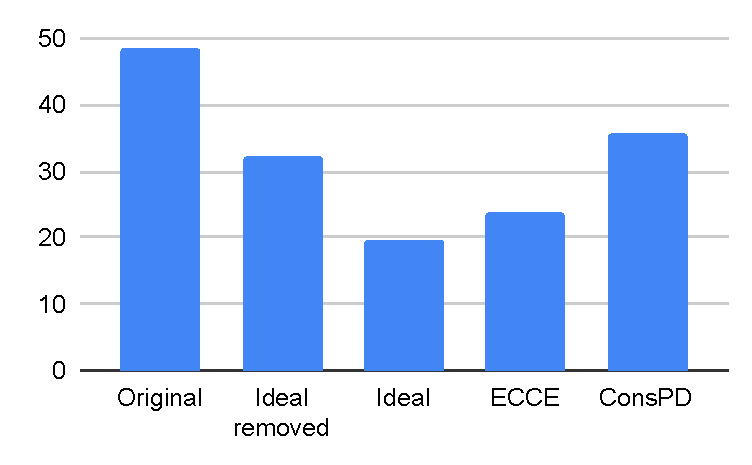
\includegraphics{graphs/maxlen.pdf}

Both \ecce and ConsPD improve performance of \lstinline{maxLength$^o$} as compared to the original program.
Removing the disjuncts with the result unified with \lstinline{^false} in the comparison relations improves the ideal program by about 40\%.
ConsPD does not perform tupling, but it does remove disjuncts which never succeed, thus its result is not as performant as the ideal program.


\subsection{Evaluator of Logic Formulas}

The relation \lstinline{eval$^o$} describes evaluation of a subset of first-order logic formulas in a given substitution.
The relation has 3 arguments.
The first argument is a list of boolean values which serves as a substitution.
The $i$-th value of the substitution is the value of the $i$-th variable.
The second argument is a formula with the following abstract syntax.
A formula is either a \emph{variable} represented with a Peano number, a \emph{negation} of a formula, a \emph{conjunction} of two formulas or a \emph{disjunction} of two formulas.
The third argument is the value of the formula in the given substitution.

We specialize the \lstinline{eval$^o$} relation to synthesize formulas which evaluate to \lstinline{^true}.
To do so, we run the specializer for the goal with the last argument fixed to \lstinline{^true}, while the first two arguments remain free variables.
Depending on the way the \lstinline{eval$^o$} is implemented, different specializers generate significantly different residual programs.

\subsubsection{The Order of Relation Calls}

One possible implementation of the evaluator is presented in listing~\ref{eval:last}.
Here the relation \lstinline{elem$^o$ subst v res} unifies \lstinline{res} with the value of the variable \lstinline{v} in the list \lstinline{subst}.
The relations \lstinline{and$^o$}, \lstinline{or$^o$}, and \lstinline{not$^o$} encode corresponding boolean operations.

\begin{figure*}[!h]
  \centering
  \begin{minipage}{0.95\textwidth}
    \begin{lstlisting}[label={eval:last}, caption={Evaluator of formulas with boolean operation last}, captionpos=b, frame=tb]
  let rec eval$^o$ subst fm res = conde [
    fresh (x y z v w) (
      (fm === var v /\ elem$^o$ subst v res);
      (fm === conj x y /\ eval$^o$ st x v /\ eval$^o$ st y w /\ and$^o$ v w res);
      (fm === disj x y /\ eval$^o$ st x v /\ eval$^o$ st y w /\ or$^o$ v w res);
      (fm === neg x /\ eval$^o$ st x v /\ not$^o$ v res))]
    \end{lstlisting}
  \end{minipage}
\end{figure*}

Note, that the calls to boolean relations \lstinline{and$^o$}, \lstinline{or$^o$}, and \lstinline{not$^o$} are placed last within each conjunction.
This poses a challenge to the CPD-based specializers such as \ecce.
Conjunctive partial deduction unfolds relation calls from left to right, so when specializing this relation for running backwards (i.e. considering the goal \lstinline{eval$^o$ subst fm ^true}), it fails to propagate the direction data onto recursive calls of \lstinline{eval$^o$}.
Knowing that \lstinline{res} is \lstinline{^true}, we can conclude that in the call \lstinline{and$^o$ v w res} variables \lstinline{v} and \lstinline{w} have to be \lstinline{^true} as well.
There are three possible options for these variables in the call \lstinline{or$^o$ v w res} and one for the call \lstinline{not$^o$}.
These variables are used in recursive calls of \lstinline{eval$^o$} and thus restrict the result of driving them.
CPD fails to recognize this, and thus unfolds recursive calls of \lstinline{eval$^o$} applied to fresh variables.
It leads to over-unfolding, big residual programs and poor performance.

The conservative partial deduction first unfolds those calls which are selected with the heuristic.
Since exploring boolean operations makes more sense, they are unfolded before recursive calls of \lstinline{eval$^o$}.
The way conservative partial deduction treats this program is the same as it treats the other implementation in which boolean operations are moved to the left, as shown in listing~\ref{eval:fst}.
This program is easier for CPD to transform which demonstrates how unequal is the behaviour of CPD for similar programs.

\begin{figure*}[!h]
  \centering
  \begin{minipage}{0.95\textwidth}
    \begin{lstlisting}[label={eval:fst}, caption={Evaluator of formulas with boolean operation second}, captionpos=b, frame=tb]
  let rec eval$^o$ subst fm res = conde [
    fresh (x y z v w) (
      (fm === var v /\ elem$^o$ subst v res);
      (fm === conj x y /\ and$^o$ v w res /\ eval$^o$ st x v /\ eval$^o$ st y w);
      (fm === disj x y /\ or$^o$ v w res /\ eval$^o$ st x v /\ eval$^o$ st y w);
      (fm === neg x /\ not$^o$ v res /\ eval$^o$ st x v))]
    \end{lstlisting}
  \end{minipage}
\end{figure*}

\subsubsection{Unfolding of Complex Relations}

Depending on the way a relation is implemented, it may take a different number of driving steps to reach the point when any useful information is derived through its unfolding.
Partial deduction tries to unfold every relation call unless it is unsafe, but not all relation calls serve to restrict the search space and thus should be unfolded.
In the implementation of \lstinline{eval$^o$} boolean operations can effectively restrict variables within the conjunctions and should be unfolded until they do.
But depending on the way they are implemented, the different number of driving steps should be performed for that.
The simplest way to implement these relations is with a table as demonstrated with the implementation of \lstinline{not$^o$} in listing~\ref{not:table}.
It is enough to unfold such relation calls once to derive useful information about variables.

\begin{figure*}[!h]
  \centering
  \begin{minipage}{0.45\textwidth}
    \begin{lstlisting}[label={not:table}, caption={Implementation of boolean \lstinline{not} as a table}, captionpos=b, frame=tb]
  let not$^o$ x y = conde [
     (x === ^true /\ y === ^false;
      x === ^false /\ y === ^true)]
    \end{lstlisting}
  \end{minipage}
\end{figure*}

The other way to implement boolean operations is via one basic boolean relation such as \lstinline{nand$^o$} which is, in turn, has a table-based implementation (see listing~\ref{not:nando}).
It will take several sequential unfoldings to derive that variables \lstinline{v} and \lstinline{w} should be \lstinline{^true} when considering a call \lstinline{and$^o$ v w ^true} implemented via a basic relation.
Conservative partial deduction drives the selected call until it derives useful substitutions for the variables involved while CPD with deterministic unfolding may fail to do so.

\begin{figure*}[!h]
  \centering
  \begin{minipage}{0.85\textwidth}
    \begin{lstlisting}[label={not:nando}, caption={Implementation of boolean operation via \lstinline{nand}}, captionpos=b, frame=tb]
  let not$^o$ x y = nand$^o$ x x y

  let or$^o$ x y z = nand$^o$ x x xx /\ nand$^o$ y y yy /\ nand$^o$ xx yy z

  let and$^o$ x y z = nand$^o$ x y xy /\ nand$^o$ xy xy z

  let nand$^o$ a b c = conde [
    ( a === ^false /\ b === ^false /\ c === ^true );
    ( a === ^false /\ b === ^true /\ c === ^true );
    ( a === ^true /\ b === ^false /\ c === ^true );
    ( a === ^true /\ b === ^true /\ c === ^false )]
    \end{lstlisting}
  \end{minipage}
\end{figure*}

\subsubsection{Evaluation Results}
In our study we considered four implementations of \lstinline{eval$^o$}:
\begin{itemize}
  \item \emph{FirstPlain} in which boolean operations are \textbf{table-based} and are placed \textbf{before} recursive calls to \lstinline{eval$^o$}
  \item \emph{LastPlain} in which boolean operations are \textbf{table-based} and are placed \textbf{after} recursive calls to \lstinline{eval$^o$}
  \item \emph{FirstNando} in which boolean operations are implemented via \lstinline{nand$^o$} and are placed \textbf{before} recursive calls to \lstinline{eval$^o$}
  \item \emph{LastNando} in which boolean operations are implemented via \lstinline{nand$^o$} andare placed \textbf{after} recursive calls to \lstinline{eval$^o$}

\end{itemize}

These four implementations are very different from the standpoint of \ecce.
We measured the time necessary to generate $1000$ formulas over two variables which evaluate to \lstinline{^true} (averaged over 10 runs).
The results are presented in table~\ref{tbl:eval}.


\begin{table}
  \centering
  \begin{tabular}{c||c|c|c|c}
                   & FirstPlain & FirstNando & LastPlain & LastNando \\ \hline\hline
  Original         & 14.8ms     & 14.5ms     & 7.4ms     & 10.1ms    \\ \hline
  \ecce            & 16.0ms     & 22.3ms     & 14.0ms    & 14.9ms    \\ \hline
  ConsPD          & 9.1ms      & 9.7ms      & 9.1ms     & 9.9ms     \\
  \end{tabular}
  \caption{Execution time of evalo}
  \label{tbl:eval}
\end{table}

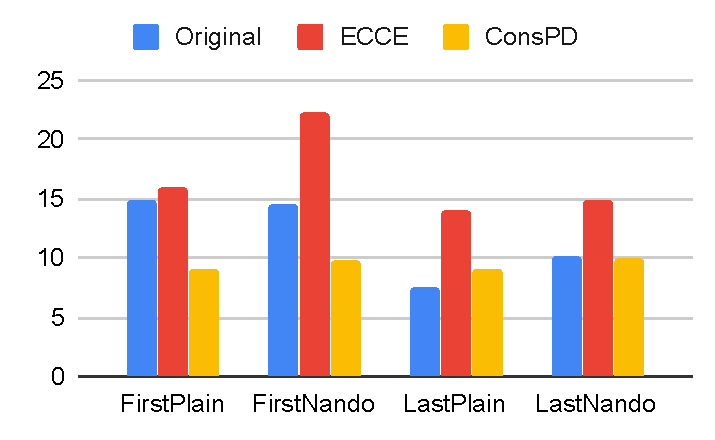
\includegraphics{graphs/prop.pdf}

ConsPD generates programs with comparable performance for all four implementations, while the quality of \ecce transformations differs significantly.
\ecce worsens performance for every implementation as compared to the original program.
ConsPD worsens performance of only the fastest implementation \emph{LastPlain}, while improving it for others.

\subsection{Unification and Path Search}

Besides evaluator of logic formulas we also run the transformers on the relation \lstinline{unify} which searches for a unifier of two terms and a relation \lstinline{isPath} specialized to search for paths in the graph.
These two relations are described in paper~\cite{lozov2019relational} so we will not go into too many details here.

The \lstinline{unify} relation was executed to find a unifier of three pairs of terms (see table~\ref{tbl:unify}) which vary in their complexity.
The original program failed to terminate on two last unification problems in under 30s, while both ConsPD and \ecce generate programs which are able to find the unifiers.

\begin{table}
  \centering
  \begin{tabular}{c||c|c|c||c}
    & \multicolumn{3}{c||}{unify} & \\
    \multirow{2}{*}{Terms} & f(X, a) & f(a \% b \% nil, c \% d \% nil, L) & f(X, X, g(Z, t)) & \multirow{2}{*}{isPath}  \\
    \cline{2-4} &
    f(a, X) & f(X \% XS, YS, X \% ZS) & f(g(p, L), Y, Y)  \\
    \hline\hline
  Original          & 0.23ms &  ---   &  ---    & 24.9ms \\ \hline
  ConsPD            & 0.07ms & 16.5ms & 397.6ms & 1.6ms  \\ \hline
  \ecce             & 0.12ms & 18.8ms & 352.0ms & 1.1ms  \\ \hline
  \end{tabular}

  \caption{Evaluation results of unification and path search}
  \label{tbl:unify}
\end{table}

The relation \lstinline{isPath} was executed to search for 3 paths of length 7 in the graph with 20 vertices and 30 edges (see table~\ref{tbl:unify}).
Both transformations significantly improve the performance as compared to the original program, although ConsPD is about 30\% worse than \ecce.


\subsection{Typechecker-Term Generator}

This relation implements a typechecker for a tiny language.
Being executed in the backward direction it serves as a generator of terms of the given type.
The abstract syntax of the language is presented below.
The variables are represented with de Bruijn indices, thus let-binding does not specify which variable is being bound.


% \begin{align*}
%   &type \ term = \\
%   &| \ BConst \ of \ Bool \\
%   &| \ IConst \ of \ Int \\
%   &| \ Var \ of \ Int \\
%   &| \ Plus \ of \ term * term \\
%   &| \ Mult \ of \ term * term \\
%   &| \ Eq \ of \ term * term \\
%   &| \ Lt \ of \ term * term \\
%   &| \ Let \ of \ term * term \\
%   &| \ If \ of \ term * term * term
% \end{align*}

\[\begin{array}{lllll}
  type \ term = &\ BConst \ of \ Bool &| \ IConst \ of \ Int &| \ Var \ of \ Int & \\
  & | \ term + term &| \ term * term &| \ term = term &| \ term < term \\
  &| \ \underline{let} \ term \ \underline{in} \ term
  &\multicolumn{2}{l}{| \ \underline{if} \ term \ \underline{then} \ term \ \underline{else} \ term} &
\end{array}\]

The typing rules are straightforward and are presented below.
Boolean and integer constants have the corresponding types regardless of the environment.
Only terms of type integer can be summed up, multiplied or checked for being less or equal.
Any terms of the same type can be checked for equality.
If-then-else expression typechecks only if its condition is of type boolean, while both then- and else-branches have the same type.
An environment $\Gamma$ is an ordered list, in which the $i$-th element is the type of the variable with the $i$-th de Bruijn index.
To typecheck a let-binding, first, the term being bound is typechecked and is added in the beginning of the environment $\Gamma$, and then the body is typechecked in the context of the new environment.
Typechecking a variable with the index $i$ boils down to getting a $i$-th element of the list.

\begin{table}
  \setlength{\tabcolsep}{0.5cm}
  \centering
  \begin{tabular}{c c}
    \infer[]{\Gamma \vdash IConst \ i : Int}{} &
    \infer[]{\Gamma \vdash BConst \ b : Bool}{} \vspace{0.5cm} \\

    \infer[]{\Gamma \vdash t + s : Int}{\Gamma \vdash t : Int, \Gamma \vdash  s : Int} &
    \infer[]{\Gamma \vdash t * s : Int}{\Gamma \vdash t : Int, \Gamma \vdash  s : Int} \vspace{0.5cm} \\

    \infer[]{\Gamma \vdash t = s : Bool}{\Gamma \vdash t : \tau, \Gamma \vdash  s : \tau} &
    \infer[]{\Gamma \vdash t < s : Bool}{\Gamma \vdash t : Int, \Gamma \vdash  s : Int} \vspace{0.5cm} \\

    \infer[]{\Gamma \vdash \underline{let} \ v \ b : \tau}{\Gamma \vdash v : \tau_v, \ (\tau_v :: \Gamma) \vdash b : \tau} &
    \infer[\Gamma \lbrack v \rbrack = \tau]{\Gamma \vdash Var \ v : \tau}{} \vspace{0.5cm} \\

    \multicolumn{2}{c}{
      \infer[]{\Gamma \vdash \underline{if} \ c \ \underline{then} \ t \ \underline{else} \ s : \tau}{\Gamma \vdash c : Bool, \Gamma \vdash t : \tau, \Gamma \vdash s : \tau}
    }


  \end{tabular}
\end{table}

We compared two possible implementations of these typing rules.
The first one is obtained by unnesting of the functional program as described in~\cite{lozov2019relational}.
The second program is hand-written in \oc.
Each implementation has been transformed with conservative partial deducer and by \ecce.

We measured the time needed to generate 100 terms of type integer (averaged over 10 iterations).
\ecce significantly worsens the execution time for both implementations.
Conservative partial deduction improves the first implementation a little bit, while worsening the performance of the second implementation 3 times.

\begin{table}
  \centering
  \begin{tabular}{c||c||c}
              & Implementation 1 & Implementation 2 \\ \hline\hline
  Original    & 0.464s           & 0.057s           \\ \hline
  ConsPD     & 0.448s           & 0.154s           \\ \hline
  \ecce        & 1.518s           & 2.543s           \\
  \end{tabular}

  \caption{Running time of generating 100 closed terms of type Int}
  \label{tbl:eval}
\end{table}

\todo{why}

\section{Conclusion}

In this paper, we discussed some issues which arise in partial deduction of a relational programming language, \mk{}.
We presented a novel approach to partial deduction which uses less-branching heuristic to select the most suitable relation call to unfold at each step of driving.
We compared this approach to the earlier implementation of conjunctive partial deduction and the implementation of CPD equipped with the new less-branching heuristic.

The conservative partial deduction improved the execution time of all relations while the implementations of CPD degraded the performance of some of them.
However, CPD equipped with the less-branching heuristic improved the execution time of one relation the most compared with the other specializers.
We conclude that there is still no one good technique which definitely speeds up every relational program.
More research is needed to develop models to predict performance of relations, these models can further be used in specialization.






\bibliographystyle{splncs04.bst}
\bibliography{bibl.bib}

\end{document}
